\documentclass{article}
\usepackage{epsfig}
\usepackage[a4paper, total={6in, 9in}]{geometry}
\begin{document}
\title{Poisson Equation in 2-D}
\author{Carl Liu}
\date{December 9 2023}
\maketitle
\newpage

The partial differential equation that was solved was 
\[\frac{\partial^2 U}{\partial x^2} +\frac{\partial^2 U}{\partial y^2} = 4\pi q(x,y)\] 
where U is the electric potential and q is the electrical charge density. The electric potential $ U= 0$ at the edge of the box. The finite difference form of the partial differential equation is 
\[\frac{U_{i+1,j} + U_{i-1,j} + U_{i,j+1} + U_{i,j-1} - 4U_{i,j}}{h^2}=4\pi q_{i,j}\]
where we have considered the large box being divided into an array of smaller  square cells, with $i,j$ as it's index. $U_{i,j}$ is the value of $U$ at the center of cell $(i,j)$, $q_{i,j}$ is the electrical charge density in cell $(i,j)$, and $h$ is the length of each cell. To simulate the boundary conditions of $U=0$, have ghost cells at the boundaries that have $U=0$ at all times. We then use the relaxation method 
\begin{enumerate}
    \item Start by rearranging the equation for $U_{i,j}$ obtaining
    \[U_{i,j} =\frac{U_{i+1,j} + U_{i-1,j} + U_{i,j+1} +U_{i,j-1}-4\pi h^2q_{i,j}}{4} \]
    \item Guess the initial electric potential $U_{i,j}^0$ for all cells. 
    \item Plug the initial guesses into the left hand side of the equation below to obtain the new estimate for $U_{i,j}$
    \[U_{i,j}^1 =\frac{U_{i+1,j}^0 + U_{i-1,j}^0 + U_{i,j+1}^0 +U_{i,j-1}^0-4\pi h^2q_{i,j}}{4} \]
    \item Repeat the process using the new estimate until convergence of $U$ is reached. In other words the change in each new estimation of $U$ is minuscule.
\end{enumerate}
We obtained as our final result after 17833 iterations, the below graph, using a $100\times 100$ grid, and charge density $q(25,25) = -4,  q(75,75) = 4$
\begin{center}
    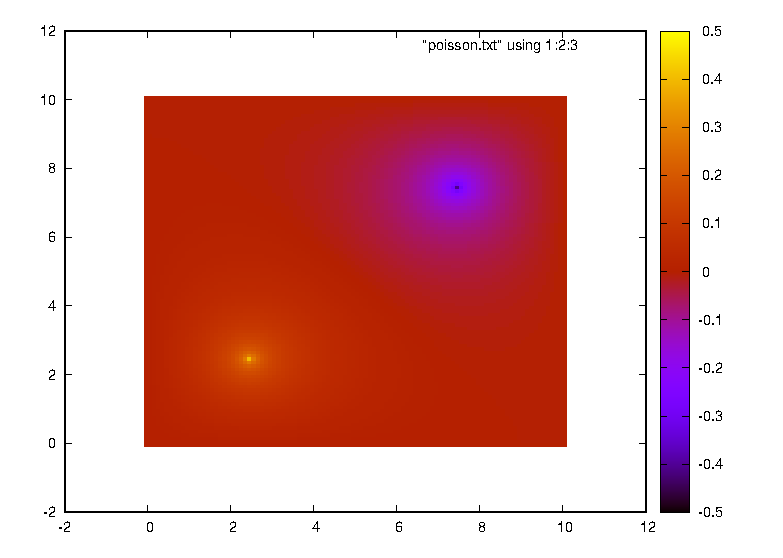
\epsfig{file=carl_liu_heatmap.eps}
\end{center}
\end{document}